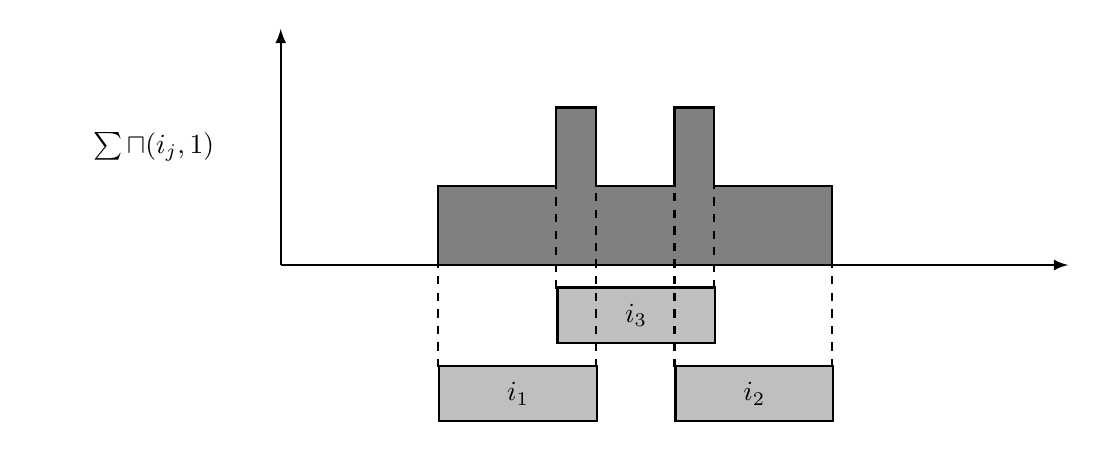
\begin{tikzpicture}
        \draw  (2,1) node[draw, thick, fill=lightgray, rectangle, anchor=south west, inner sep=0pt, minimum width=2cm, minimum height=0.7cm] {\textbf{$i_1$}};
        \draw  (5,1) node[draw, thick, fill=lightgray, rectangle, anchor=south west, inner sep=0pt, minimum width=2cm, minimum height=0.7cm] {\textbf{$i_2$}};
        \draw  (3.5,2) node[draw, thick, fill=lightgray, rectangle, anchor=south west, inner sep=0pt, minimum width=2cm, minimum height=0.7cm] {\textbf{$i_3$}};
        \draw[thick, -latex] (0,3) -- (0,6) node[midway, left, minimum width=3.2cm] {$\sum \sqcap(i_j, 1)$};

        \draw[thick, fill=gray] (2,3) -- (2,4) -- (3.5,4) -- (3.5,5) -- (4,5) -- (4,4) -- (5,4) -- (5,5) -- (5.5,5) -- (5.5,4) -- (7,4) -- (7,3);
        \draw[thick, dashed] (2,1.7) -- (2,3);
        \draw[thick, dashed] (3.5,2.7) -- (3.5,4);
        \draw[thick, dashed] (4,1.7) -- (4,4);
        \draw[thick, dashed] (5,1.7) -- (5,4);
        \draw[thick, dashed] (5.5,2.7) -- (5.5,4);
        \draw[thick, dashed] (7,1.7) -- (7,3);
        \draw[thick, -latex] (0,3) -- (10,3);
    \end{tikzpicture}
